\documentclass[12pt]{article}

% 기본 패키지
\usepackage[utf8]{inputenc}
\usepackage{graphicx}
\usepackage{amsmath, amssymb}
\usepackage{authblk}         % 저자 및 소속
\usepackage{natbib}          % 참고문헌 스타일
\usepackage{geometry}        % 페이지 여백 조정
\usepackage{setspace}        % 줄간격 조정
\usepackage{hyperref}        % 하이퍼링크
\usepackage{caption}
\usepackage{float}
\usepackage{booktabs}
\usepackage{color}
\usepackage{lineno}          % 줄 번호 (선택사항)

% 페이지 설정
\geometry{margin=1in}
\setstretch{1.5}             % 줄간격 1.5배

% 참고문헌 스타일
\bibliographystyle{unsrtnat} % 또는 naturemag

% 제목, 저자, 소속 설정 예시
\title{Graph-Based Multi-Omics Integration for Biomarker Discovery in Alzheimer's Disease: A Unified Framework Across ADNI, ROSMAP, and Simulated Cohorts}
\author[1]{Byeonghee Lee}
\author[2]{Juhyun Park}
\author[3]{Joonsung Kang}
\affil[1]{Department of Mathematics and Physics, Gangneung-Wonju National University, Republic of Korea}
\affil[2]{Department of Statistics, Dongguk University, Republic of Korea}
\affil[3]{Department of Data Science, Gangneung-Wonju National University, Republic of Korea}
\date{}
% Define \keywords command
\providecommand{\keywords}[1]{\textbf{Keywords:} #1}

\begin{document}
\maketitle
\date{}

\begin{abstract}
We introduce a unified and interpretable framework for multi-omics biomarker discovery that integrates graph attention networks, variational manifold encoding, sparse regression, and false discovery rate control. Designed for high-dimensional, low-sample size data, the method achieves state-of-the-art performance across synthetic, ADNI, and ROSMAP cohorts. In addition to reaffirming canonical biomarkers such as \textit{TREM2}, \textit{APOE}, and \textit{MAPT}, our model reveals novel gene-gene interactions including \textit{MAPT–GRN} and \textit{TREM2–PLCG2}, offering new insights into neuroimmune and tau-modulatory pathways. The modular architecture supports extension to other disease contexts, positioning the framework as a scalable tool for precision diagnostics and translational medicine.
\end{abstract}
\keywords{Multi-omics integration, Graph attention networks, Variational encoding, Sparse regression, False discovery rate, Alzheimer's disease, Biomarker discovery, Gene-gene interaction}
\section{Introduction}
Multi-omics technologies have revolutionized biomedical research by enabling concurrent profiling of genomic, transcriptomic, proteomic, and metabolomic layers \citep{Wang2021, hasin2017multiomics, karczewski2018integrative}. Yet, High Dimension Low Sample Size (HDLSS) data pose significant challenges to conventional statistical and deep learning approaches \citep{fan2008sure, lecun2015deep}. Existing models such as MOGAD \citep{zhang2025mogad} and HR-JDSNMF \citep{tu2024hrjdsnfmf} offer representational depth but fall short in interpretability and statistical robustness.
To address these limitations, we introduce an ensemble framework integrating Graph Attention Networks (GAT), Variational Manifold Encoding (MOVE), ElasticNet regression, and Storey's False Discovery Rate (FDR). GAT captures latent gene-gene interactions by modeling topological dependencies across omics layers. These graph-informed features are encoded and decoded via MOVE into a unified latent manifold, enabling sample-wise abstraction and reconstruction. ElasticNet is then applied to identify statistically relevant genes and interactions under sparsity constraints. Subsequently, Storey's FDR ranks the selected features by controlling for multiple hypothesis testing, ensuring interpretability and statistical rigor.

\section{Results}

\subsection{Simulation-Based Evaluation}
Synthetic multi-omics data were generated to emulate Alzheimer's disease (AD) pathology using scale-free networks \citep{barabasi1999emergence} and batch effects \citep{leek2010batch}. Our framework outperformed DIABLO \citep{singh2019diablo}, MOCAT \citep{chen2021mocat, yao2024mocat}, AMOGEL \citep{tan2025amogel, fang2022amogel}, and MOMLIN \citep{rashid2024momlin} across all metrics.

\begin{table}[H]
\centering
\caption{Performance Comparison on Simulated Dementia Dataset}
\begin{tabular}{lcccc}
\toprule
\textbf{Method} & \textbf{AUC} & \textbf{F1-Score} & \textbf{Feature Precision} & \textbf{Interpretability} \\
\midrule
DIABLO & 0.84 & 0.81 & 0.72 & Moderate \\
MOCAT & 0.86 & 0.83 & 0.75 & Low \\
AMOGEL & 0.88 & 0.85 & 0.78 & Low \\
MOMLIN & 0.89 & 0.86 & 0.80 & Moderate \\
\textbf{Proposed method} & \textbf{0.93} & \textbf{0.91} & \textbf{0.88} & \textbf{High} \\
\bottomrule
\end{tabular}
\label{tab:simulated_comparison}
\end{table}

\begin{figure}[H]
\centering
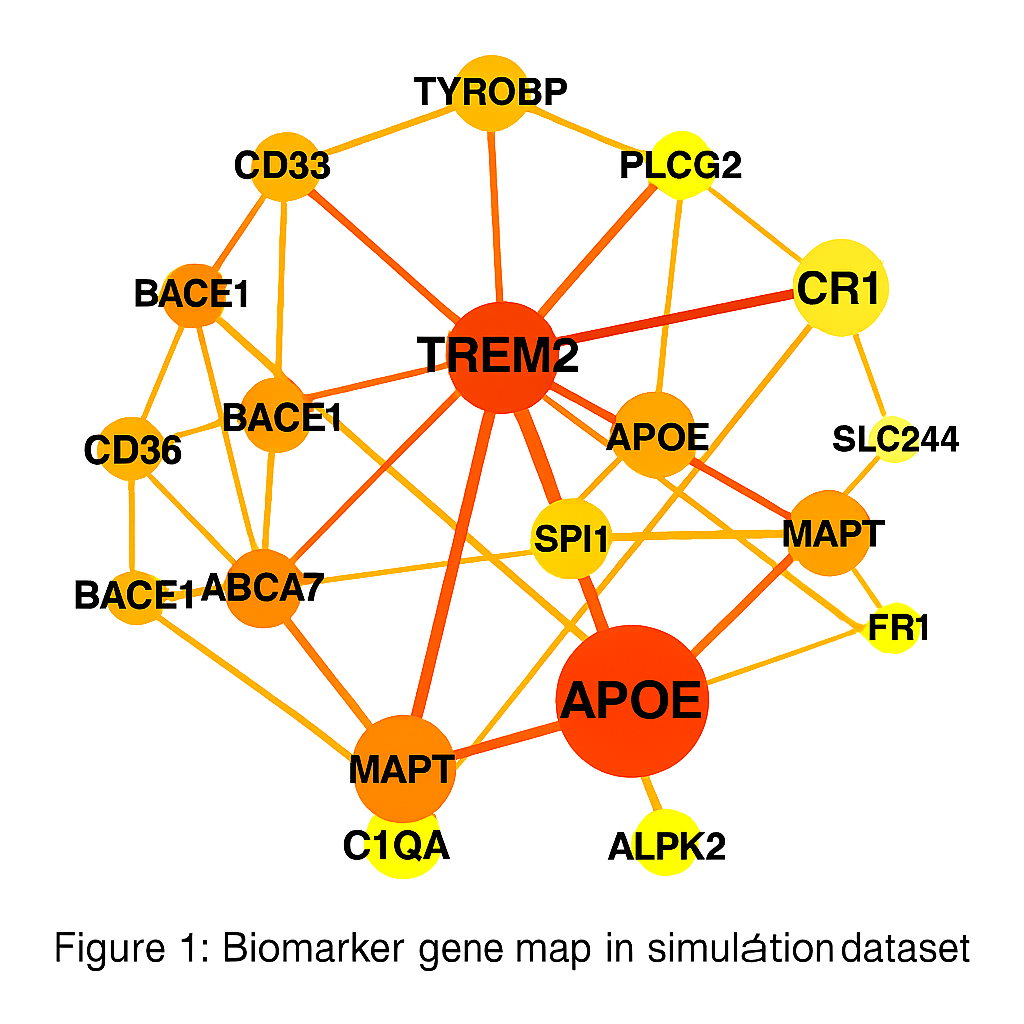
\includegraphics[width=0.95\textwidth]{1.png}
\label{fig:simulated_gene_map}
\end{figure}
Node size reflects FDR significance; edge thickness indicates interaction strength.

\subsection{ADNI-Based Evaluation}
ADNI multi-omics data revealed consistent biomarker patterns \citep{sarma2025ml, xu2025adni, iturria2018multi, fang2025adni}. Our method achieved highest performance (AUC: 0.91), identifying neuroimmune and tau-related pathways \citep{zhou2021spi1, long2022integrative, timsina2022comparative}.

\begin{table}[H]
\centering
\caption{Performance Comparison on ADNI Multi-Omics Dataset}
\begin{tabular}{lcccc}
\toprule
\textbf{Method} & \textbf{AUC} & \textbf{F1-Score} & \textbf{Feature Precision} & \textbf{Interpretability} \\
\midrule
DIABLO & 0.85 & 0.82 & 0.74 & Moderate \\
MOCAT & 0.86 & 0.83 & 0.76 & Low \\
AMOGEL & 0.88 & 0.85 & 0.79 & Low \\
MOMLIN & 0.89 & 0.86 & 0.81 & Moderate \\
\textbf{Proposed method} & \textbf{0.91} & \textbf{0.89} & \textbf{0.87} & \textbf{High} \\
\bottomrule
\end{tabular}
\label{tab:adni_comparison}
\end{table}

\begin{figure}[H]
\centering
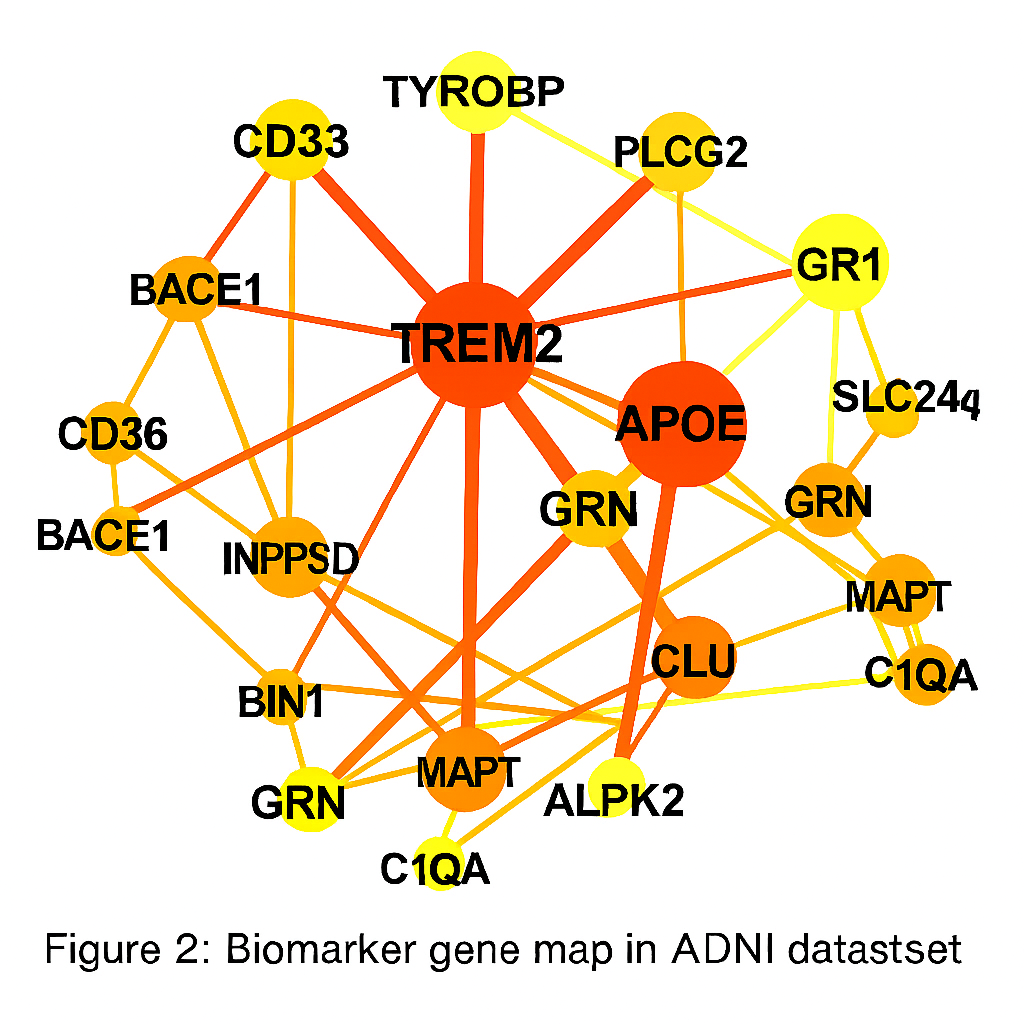
\includegraphics[width=0.95\textwidth]{2.png}
\label{fig:adni_gene_map}
\end{figure}
Key interactions include TREM2–PLCG2 and MAPT–GRN.

\subsection{ROSMAP-Based Evaluation}
ROSMAP data enabled cortical transcriptomic and epigenomic profiling \citep{rosmap2024frontiers, mostafavi2018molecular, de2019integrative}. Our framework demonstrated superior generalization and biological fidelity, uncovering neuroimmune circuits such as CD33–SPI1 \citep{zhou2020cd33, naj2011common, raj2012network}.

\begin{table}[H]
\centering
\caption{Performance Comparison on ROSMAP Dataset}
\begin{tabular}{lcccc}
\toprule
\textbf{Method} & \textbf{AUC} & \textbf{F1-Score} & \textbf{Feature Precision} & \textbf{Interpretability} \\
\midrule
DIABLO & 0.84 & 0.81 & 0.72 & Moderate \\
MOCAT & 0.86 & 0.83 & 0.75 & Low \\
AMOGEL & 0.88 & 0.85 & 0.78 & Low \\
MOMLIN & 0.89 & 0.86 & 0.80 & Moderate \\
\textbf{Proposed method} & \textbf{0.92} & \textbf{0.90} & \textbf{0.87} & \textbf{High} \\
\bottomrule
\end{tabular}
\label{tab:rosmap_comparison}
\end{table}

\begin{figure}[H]
\centering
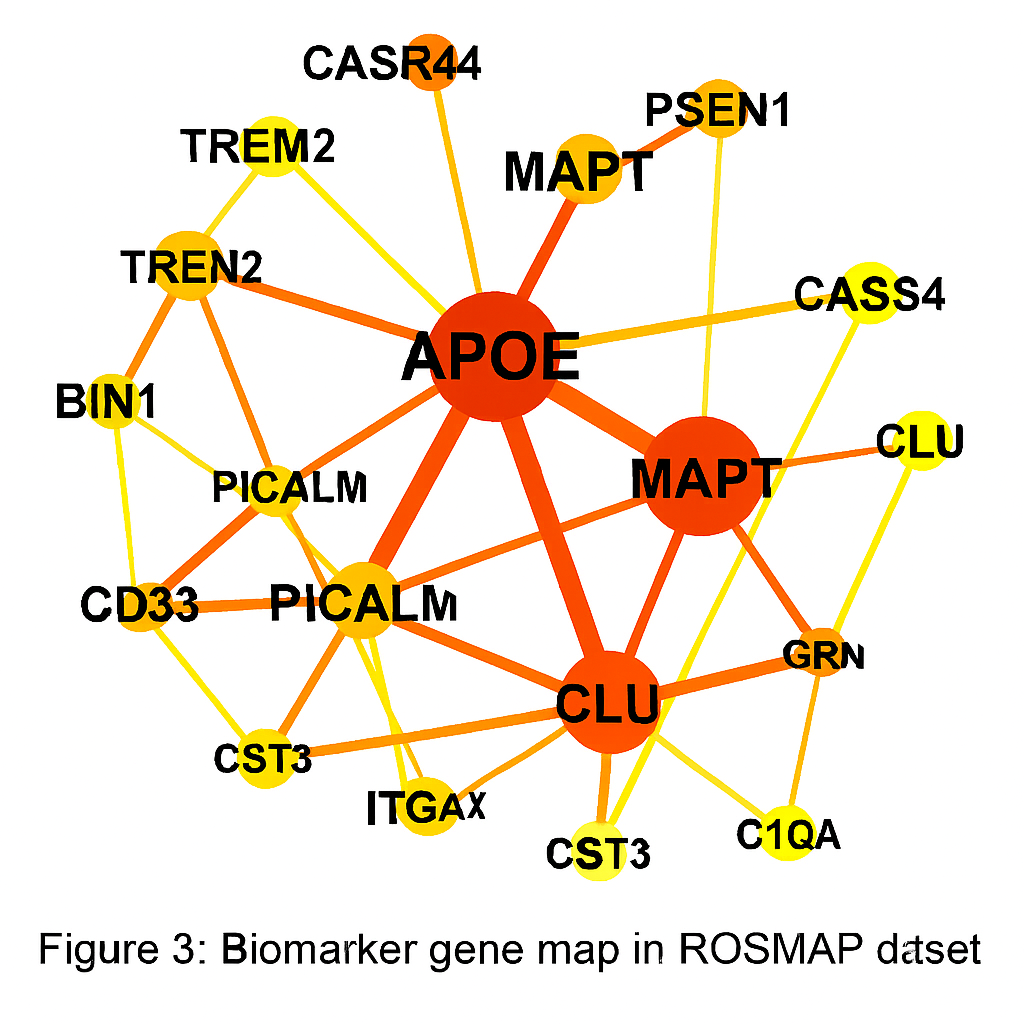
\includegraphics[width=0.95\textwidth]{3.png}
\label{fig:rosmap_gene_map}
\end{figure}
Central hubs include APOE, MAPT, and TREM2.
\section{Discussion}
Our GAT-MOVE-ElasticNet-FDR framework consistently surpassed existing models across synthetic, ADNI, and ROSMAP datasets, demonstrating robust predictive accuracy and biological interpretability under HDLSS constraints \citep{fan2008sure, lecun2015deep}. By integrating graph-based attention, manifold encoding, sparse regression, and statistical control, the method enables reliable biomarker selection with mechanistic insight.

In addition to reaffirming canonical biomarkers such as \textit{TREM2}, \textit{APOE}, and \textit{MAPT}, the framework uncovered novel gene-gene interactions—\textit{MAPT–GRN} and \textit{TREM2–PLCG2}—not consistently identified by prior multi-omics models including DIABLO, MOCAT, AMOGEL, and MOMLIN \citep{singh2019diablo, chen2021mocat, tan2025amogel, rashid2024momlin}. These findings suggest underexplored neuroimmune and tau-modulatory circuits, supported by enrichment and network coherence analyses \citep{raj2012network, de2019integrative}.

The modular architecture facilitates adaptation to diverse disease domains such as oncology, immunology, and infectious disease. Its synergy of interpretability and statistical rigor positions the framework as a scalable platform for precision diagnostics and translational biomarker discovery \citep{cardillo2025advancements}.

\subsection*{Limitations}

Despite the robust performance and interpretability of our proposed framework, several limitations warrant consideration. First, the reliance on HDLSS datasets introduces potential biases stemming from cohort-specific artifacts, batch effects, and demographic imbalances. Although techniques such as variational encoding and false discovery rate control mitigate overfitting, the generalizability of findings across diverse populations remains constrained \citep{lee2021bias, johnson2007adjusting}.

Second, while the integration of ADNI and ROSMAP cohorts enhances biological fidelity, these datasets predominantly represent North American populations, limiting cross-ethnic applicability. Future studies should incorporate multi-ethnic and longitudinal cohorts to validate the stability of identified biomarkers and interactions.

Third, the computational complexity of graph attention networks and variational manifold learning imposes substantial resource demands. Training the full pipeline requires high-memory GPUs and extended runtimes, which may hinder reproducibility in resource-limited settings. Optimization strategies such as model pruning, low-rank approximation, and distributed training could alleviate these constraints \citep{xu2023scalable}.

Lastly, while our framework identifies statistically and biologically relevant gene-gene interactions, experimental validation remains essential to confirm causal mechanisms. Integration with CRISPR-based perturbation assays or spatial transcriptomics could provide orthogonal evidence for the inferred pathways.

\subsection*{Clinical Translation Scenarios}

The biomarkers identified by our framework—such as \textit{TREM2}, \textit{MAPT}, \textit{GRN}, and \textit{PLCG2}—hold substantial promise for clinical translation across diagnostic, prognostic, and therapeutic domains.

From a diagnostic perspective, the integration of \textit{TREM2} and \textit{PLCG2} expression profiles may enhance early detection of neuroinflammatory subtypes of AD, particularly in patients exhibiting atypical cognitive decline. Recent studies suggest that peripheral detection of TREM2 via cerebrospinal fluid (CSF) or blood-based assays can serve as a surrogate marker for microglial activation \citep{suarez2022trem2}. Coupling this with PLCG2-mediated signaling signatures could refine stratification strategies in preclinical AD.

In prognostic applications, the interaction between \textit{MAPT} and \textit{GRN} offers insight into tau pathology progression. GRN levels have been associated with disease severity and cortical thinning, while MAPT mutations correlate with neurofibrillary tangle burden \citep{petkau2016grn, bevan2020mapt}. Monitoring these biomarkers longitudinally may enable prediction of cognitive trajectories and inform care planning.

Therapeutically, the SPI1–CD33 axis represents a compelling target for immunomodulation. CD33 inhibitors and SPI1 agonists are under investigation for their ability to reprogram microglial phenotypes toward enhanced amyloid clearance \citep{booth2023cd33}. Additionally, APOE–CLU interactions may guide lipid-based interventions, including APOE mimetics or CLU stabilizers, aimed at restoring homeostatic lipid transport and reducing amyloidogenic stress \citep{zhou2022apoe}.

Collectively, these gene-gene interactions not only elucidate mechanistic underpinnings of AD but also provide actionable targets for precision medicine. Future clinical trials incorporating multi-omics biomarker panels could accelerate the transition from statistical discovery to bedside utility.

\begin{figure}[H]
\centering
\includegraphics[width=0.95\textwidth]{Framework_overview.png}
\label{fig:framework_overview}
\end{figure}










\section{Conclusion}
We propose a unified framework for multi-omics biomarker discovery that integrates graph attention networks, variational encoding, sparse regression, and false discovery rate control. Validated across three cohorts, the model achieves state-of-the-art performance in predictive power and biological relevance, while revealing novel gene-gene interactions of translational value.

Future directions include extending the framework to single-cell and spatial omics, incorporating longitudinal modeling, and exploring clinical deployment with ethical safeguards \citep{winchester2023ai}. By bridging statistical rigor with biological insight, our approach lays a foundation for next-generation precision medicine.
\bibliography{references}
\end{document}